\begin{Q}
\textbf{\Large K-Means 1}\\

\begin{enumerate}

\item Mention if K-Means is a supervised or an un-supervised method and state the reason.\\
\textbf{Asnwer\: un-supervised}, since with kmean there is no requirement to label data of anysort, rather the algorithm is rather simply just clustering data together and dealing with distortion.

\item Assume that you are trying to cluster data points $x_{i}$  for $ i \in \{1,2, \dots, D\}$ into $K$ clusters each with center $\mu_{k}$  where $ k \in \{1,2, \dots, K \}$. The objective function for doing this clustering involves minimization of the Euclidean distance between the points and the cluster centers. It is given by  \begin{equation*}
\min\limits_{\mu} \min\limits_{r}\sum\limits_{i \in D} \sum\limits_{k =1}^{K} \frac{1}{2} r_{ik} \|x_{i} -\mu_{k}\|_{2}^{2}. \\
 \end{equation*} \\ How do you ensure hard assignment of one data point to one and only one cluster at a given time?
 
 \textbf{Hint:} By hard assignment we mean that you are 100 \% sure that a point either belongs or doesn't belong to a cluster.\\
\textbf{Answer:} to best ensure that we are 100\% certain about what cluster a point belongs to we look to see what cluster minimizes its distance to the point and if it just so happens that a point is equdistance from multiple cluster then we simply just take the first cluster presented
 
 \item How does your answer to part b change if we want to obtain a soft assignment instead?
 
 \textbf{Hint:} By soft assignment we mean that  a point  belongs to a cluster with some probability.\\
\textbf{Answer:}If we were to use soft clustering then we could use percentages and probability where a point would stores a the likelihood that its near a certain cluster since we no longer have to worry about beign set to one main cluster, but rather the likelyhood of being in a cluster. This leaves us with less ambiguity as to what to do with points that have clusters with equal probability since they can belong to multiple.
 
 \item Looking at the following plot, what is the best choice for the number of clusters?
 \begin{center}
 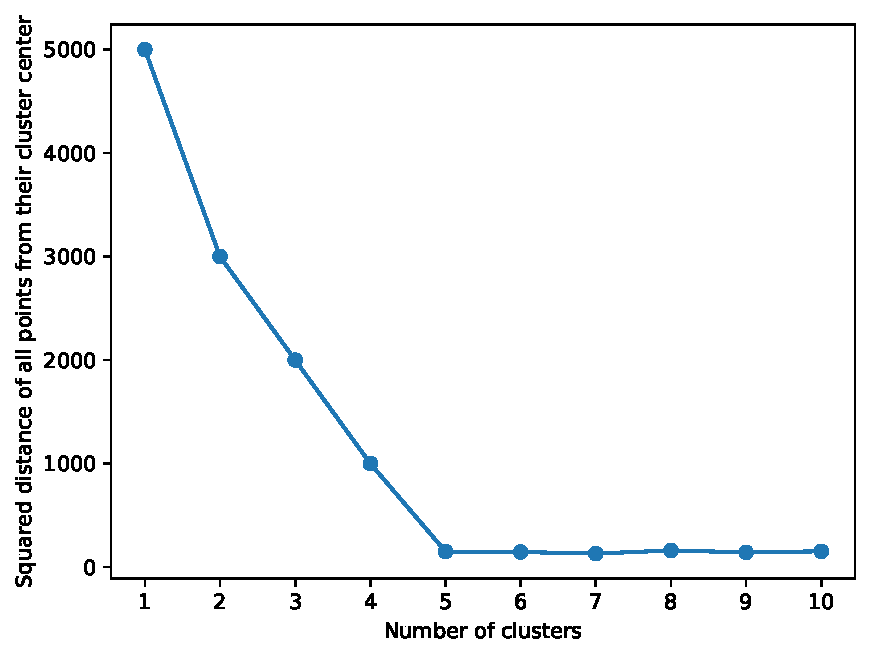
\includegraphics[width=8cm]{figs/cluster.pdf}
 \end{center}
 \textbf{Answer:} since after 5 clusters and onward the spread from the cluster center seems to level out the best choice is 5 clusters.
 
 \item Would K-Means be an efficient algorithm to cluster the following data? Explain your answer in a couple of lines.
 \begin{center}
 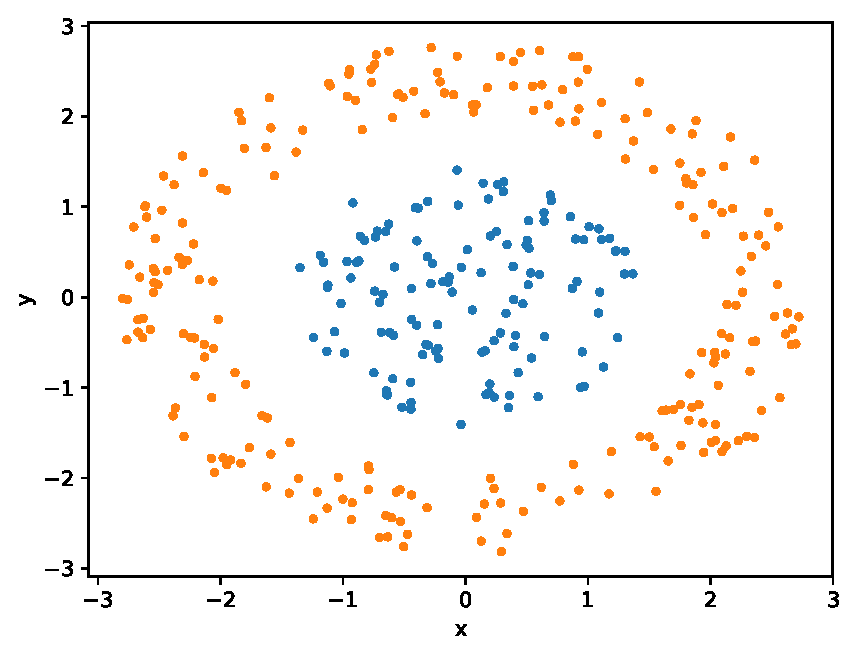
\includegraphics[width=8cm]{figs/concentric.pdf}
 \end{center}
 \textbf{Answer:} No, since trying to classify the data into two distinct groups would require multiple groups. The overall mean of all the datapoints is the center of the and trying to tether the outter ring to a single cluster would be hard for that reason it is unreasonable to use k-mean clustering for this data

\end{enumerate}


\end{Q}
          